\section{CARLA Simulator}

\acrfull{carla} is an open-source photo-realistic simulator for autonomous driving research \cite{introducing-carla-paper}. It was developed from the ground up to support development, training and validation of autonomous urban driving systems. CARLA provides free open digital assets such as urban layouts, buildings and vehicles. Additionally the simulator includes a suit of sensors, environmental conditions, full control over of static and dynamic actors, a traffic manager and more.

CARLA is built with a scalable client-server architecture in mind. The server uses Unreal Engine \cite{unrealengine} as a simulation foundation and is responsible for tasks such as scene and sensor rendering, computation of realistic physics, actor updates and providing updated world information to the connected clients. Multiple clients can be connected to the CARLA server, and these send commands to the server and receive updated world information in return. Example commands are traffic generation, spawning new actors, controlling vehicles and setting weather conditions.

\subsection{Python API}
To implement the client-server functionality, the CARLA team has developed client APIs in Python \cite{carla-python-api} and C++ \cite{carla-cplusplus-api} that leverages sockets to establish a connection to the server. The work in this project is based on the latest released version of the Python API, which in the time of writing is version 0.9.14. The Python API can be used to control the core parts of the simulation: 

\begin{description}
    \item[World:] The world represents the simulation, and one can change properties such as weather conditions, lighting and the map to use.
    \item[Map:] The map represents the actual simulated world, often called the town. The client can manage roads, lanes and junctions in the map, which are used together with waypoints to provide vehicles with a navigation path. Waypoints are simply points in 3D space oriented in the direction of the lane containing it.
    \item[Actors:] An actor is anything that plays a role in the simulation. Examples are pedestrians, vehicles, sensors and traffic lights.
    \item[Blueprints:] Blueprints are already-made models used to spawn new actors into the world. These includes properties such as vehicle color, sensor channels and pedestrian walking speed.
    \item[Sensors:] Sensors are attached to vehicles. They observe the simulated environment, collect data and make this available to the client. Many sensor types exists in CARLA, including realistic sensors (cameras, \acrshort{lidar}, GPS, etc.) and ground-truth sensors from the simulator (collision detection, semantic segmentation, etc.). 
\end{description}


\subsection{Leaderboard}
The CARLA Autonomous Driving Leaderboard \cite{carla-leaderboard} is an open platform for evaluation of driving performance by autonomous agents in realistic traffic scenarios. The goal of the platform is to simplify comparisons between different approaches to autonomous driving using a set of predefined routes. The routes vary in weather conditions and world layouts, and contain scenarios such as lane merging, lane changing, intersections, yielding to emergency vehicles and handling traffic lights. They also have constraints on which type of sensors one can utilize, depending on which leaderboard track they belong to. There are two leaderboard tracks; the "SENSORS track" only allows access to sensors attached to the vehicles, while the "MAP track" allows access to an HD world map in addition to the sensors.

The evaluation is based on two metrics. The first is route completion, which simply is the average percentage of route distance completed. The other metric counts infractions per kilometer and aggregates them into a penalty score. The infraction types counted by the leaderboard are collisions with pedestrians, vehicles and static objects, as well as running red lights and stop signs. The route completion score and infraction score is combined into a driving score, which is the main metric of the leaderboard.

There are two versions of the leaderboard. Leaderboard 1.0 is for CARLA version 0.9.10, while Leaderboard 2.0 is for the latest CARLA version (0.9.14). Although Leaderboard 2.0 is the current version, it contains no entries at the time of writing. This report will therefore discuss submissions from Leaderboard 1.0.


\subsection{Alternatives to CARLA}
There exists multiple simulator alternatives to CARLA, each with their own advantages and disadvantages. They often have a trade-off between visual fidelity of the simulated 3D environment and the level of realism in the computed vehicle physics. According to \textcite{carla-an-inside-out}, who have done an extensive comparison between different alternatives, the state-of-the-art simulators that best meet this trad-off are CARLA and LGSVL \cite{LGSVL-simulator}. Similarly to CARLA, the open source LGSVL simulator provides tools which allows users to customizes sensors, controllable objects and other modules. Additionally, LGSVL provides integration with autonomous driving software which makes it a fully end-to-end tool. Note that the simulator stopped receiving updates by original authors as of January 2022. There still exist usable forks of the project which can be used, however. Other popular open source alternatives are AirSim \cite{airsim}, DeepDrive \cite{deepdrive} and Torcs \cite{torcs}.

An interesting upcoming simulator is NVIDIA Drive Sim \cite{nvidia-drive-sim}. It is an end-to-end simulation platform with focus on being physically accurate, fast and efficient at scale. While this is a project showing impressive photo realistic simulation, it is currently in an early access phase, meaning you need to apply to access it. Another disadvantage is the commercial and closed nature of the product, meaning that one will have less control and configurability over the simulator.

% kun CARLA finnes på paperswithcode

\subsection{Ways to run the CARLA server}

The primary way to use the CARLA server is by downloading and installing the packaged version of the simulator\footnote{\url{https://carla.readthedocs.io/en/0.9.14/start_quickstart/}}. The packaged version is not customizeable. One can also build CARLA from the source code\footnote{\url{https://carla.readthedocs.io/en/0.9.14/build_carla/}}. This is the recommended approach if one wants to add extra features, assets or maps to the simulator via Unreal Editor. CARLA can be built from source on Linux and Windows. The last option is to run the simulator in a Docker container\footnote{\url{https://carla.readthedocs.io/en/0.9.14/build_docker/}}. This is useful for running without a display and for running multiple servers with GPU mapping. Different versions of CARLA support different graphics APIs. Versions until 0.9.11 supports using both Vulkan and OpenGL, but only OpenGL worked for us when running without a display. Versions equal to and after 0.9.12 only support Vulkan, and worked both with and without a display connected. We used the Docker approach for all our tasks except when adding a custom vehicle, as this required a version of CARLA built from source with access to Unreal Editor. This is explained in more detail in \cref{sec:custom-vehicle}.

\subsection{Graphical differences between CARLA versions 0.9.10 vs 0.9.14}
At the time of writing, the top submissions on the CARLA Leaderboard are based on CARLA version 0.9.10. There is however a significant graphical difference between version 0.9.10 and the latest versions. \cref{fig:10-vs-14} showcases this. The primary reason for the differences is the upgrade to Unreal Engine 4.26 in CARLA version 0.9.12. The upgrade gave a much improved lighting engine which is especially noticeable in darker scenarios. 
\todo{Reformulere dette?} As our thesis works towards closing the gap between simulation and reality, we therefore wanted to utilize the more realistic environment found in version 0.9.14. We also noticed some graphical glitches when running CARLA version 0.9.10 without a display with OpenGL in Docker (\cref{fig:black dots}). This was an know issue with OpenGL and Linux in version 0.9.10 \cite{github-rendering-issues-0.9.10}, and in order to use Vulkan with Docker without a display we had to move to upgrade the CARLA version.

\begin{comment}
    - forklare hvorfor vi bruker to versjoner in the first place
        - unngå graphical glitches, mindre gap mellom sim og reality
    - bedre lighting engine --> mørkere maps --> vanskelig uten headlights
    - svarte prikker/flekker på kameratet
    - additional maps innebygd i carla docker 0.9.14
\end{comment}

\begin{figure}[htbp]
    \centering
    
    \begin{subfigure}[b]{0.6\textwidth}
        \centering
        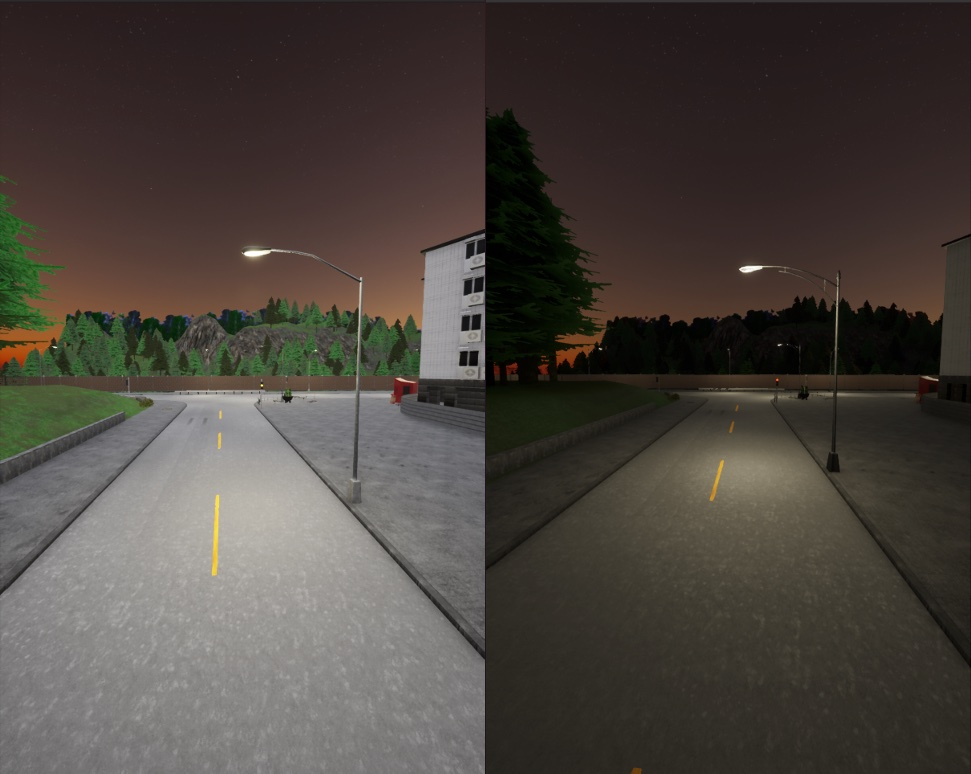
\includegraphics[width=\textwidth]{chapters/2-background/figures/10-vs-14-1.jpeg}
        \label{fig:10-vs-14-1}
    \end{subfigure}

    \begin{subfigure}[b]{0.6\textwidth}
        \centering
        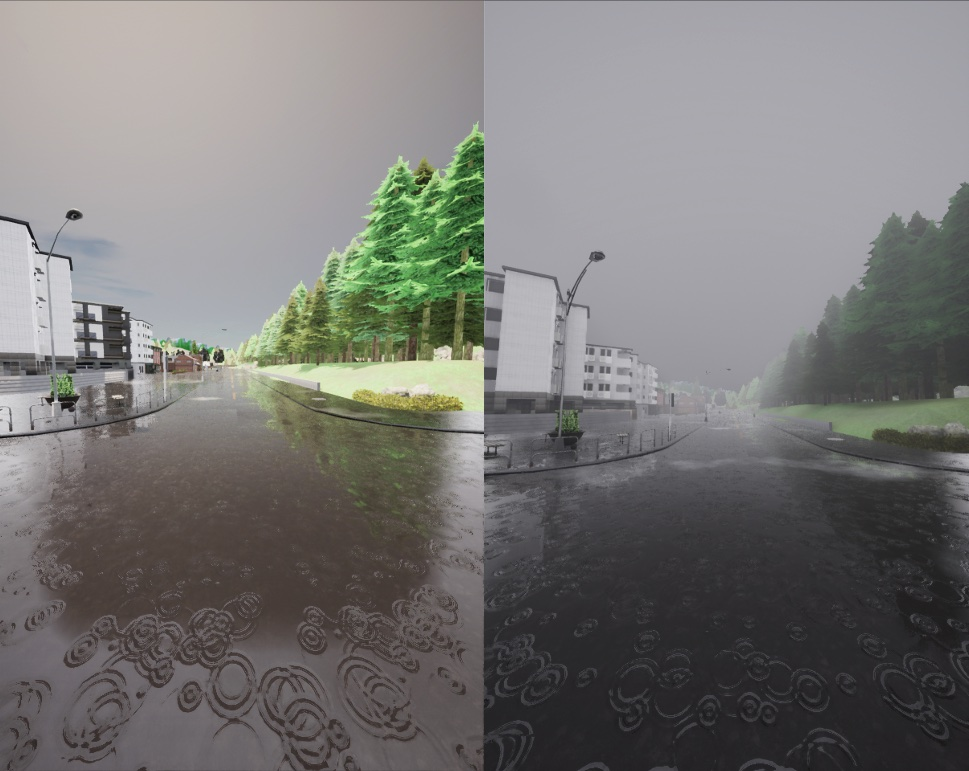
\includegraphics[width=\textwidth]{chapters/2-background/figures/10-vs-14-2.jpeg}
        \label{fig:10-vs-14-2}
    \end{subfigure}
    
    \begin{subfigure}[b]{0.6\textwidth}
        \centering
        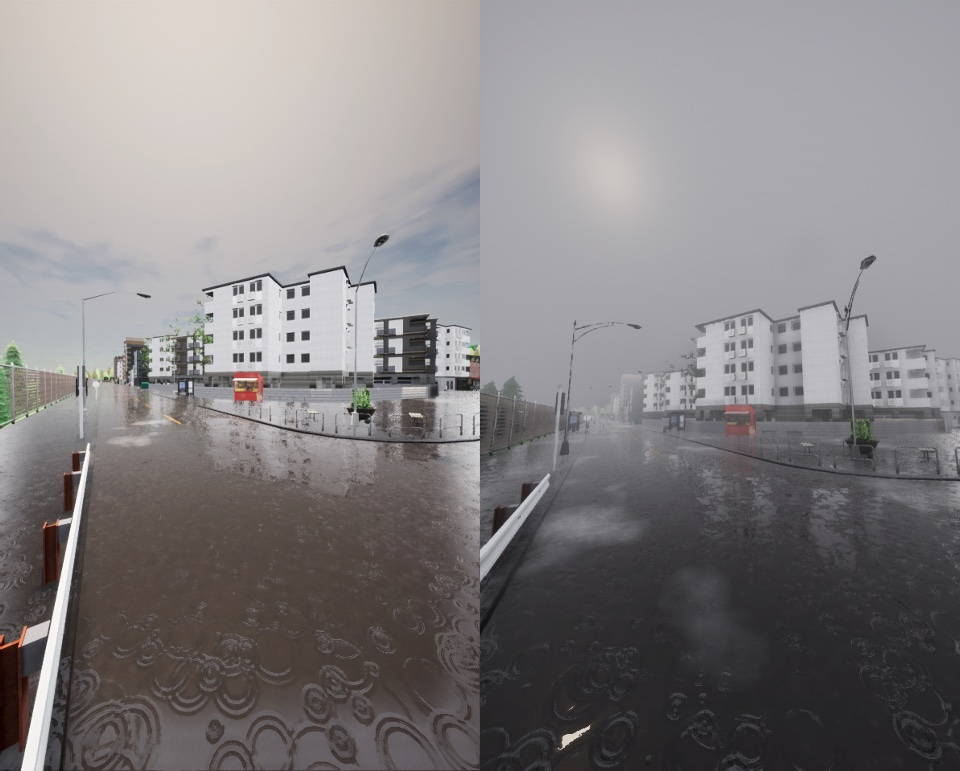
\includegraphics[width=\textwidth]{chapters/2-background/figures/10-vs-14-3.jpeg}
        \label{fig:10-vs-14-3}
    \end{subfigure}
    
    \caption{Three examples comparing the graphical differences between CARLA versions 0.9.10 (left) and 0.9.14 (right).
    In general, there is less ambient lighting and fog is more dense.
    Additionally, CARLA 0.9.14 features a new effect where rain drops on the camera lens can distort parts of the image (lower right).
    }
    \label{fig:10-vs-14}
\end{figure}

\begin{figure}[htbp]
    \centering
    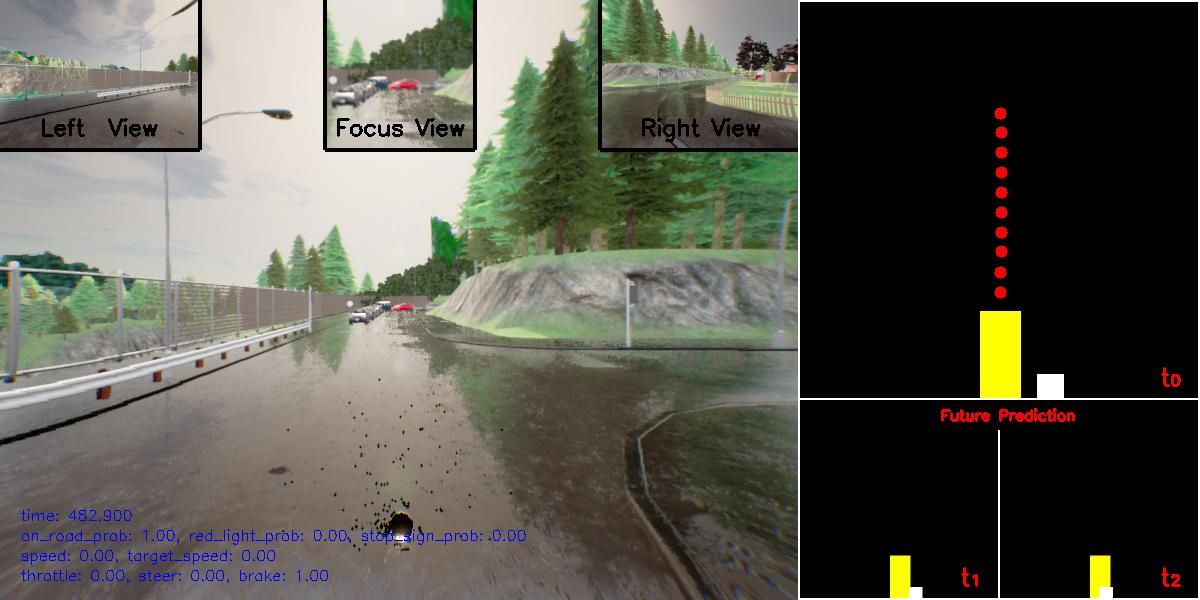
\includegraphics[width=\textwidth]{chapters/2-background/figures/black-dots.jpg}
    \caption{Running CARLA version 0.9.10 with OpenGL in Docker resulted in graphical glitches in the form of black dots on the cameras. The black dots can be seen in the bottom center of the left image. In this example one can see that the model thinks the road in front is blocked (the red circles in the top right image).}
    \label{fig:black dots}
\end{figure}